\documentclass{article}
\usepackage{epsfig}
\usepackage{amsfonts}
\usepackage{srcltx} % used by WinEdt
\usepackage{authblk}


\begin{document}
\title{CS463 Project Report (Spring 2021)}

\author[1]{Author A (AM 001)\thanks{A.A@university.edu}}
\author[2]{Author B (AM 002)\thanks{B.B@university.edu}}
\affil[1]{Department of Computer Science, University of Crete}
\affil[2]{Department of Mechanical Engineering, \LaTeX\ University}



\maketitle



%----------------------
\section{Introduction}


Guidelines:
\begin{itemize}
 \item Describe exactly what you have done  and the results of the experimental evaluation.
\item  Mention explicitly what you {\em have not done}, or whatever extra feature you have implemented.
\item  You could also mention the strong and weak points of your project.
\item  Describe the work that has been done by each individual  member of the team
\item  Structure your report to sections and subsections.
\end{itemize}




This report is structured as follows:
Section \ref{sec:E} discusses ....
Finally
Section \ref{sec:Conclusion} concludes the report.


%------------------------------------------
\section{Titlos Enothtas}
\label{sec:E}

\subsection{Titlos Ypoenotitas}


Based on the results of \cite{Rochio} we ...


\subsection{Titlos Ypoenotitas}


Examples of math symbols


\[
sim_{\cos}(D_i,D_j) = \cos (\vec{D_i}, \vec{D_j})
\]


\begin{eqnarray}
   w_{i,j}      &=& TF(i,j) * IDF_i \\
   TF(i,j)      &=& \frac { freq_{i,j} } { max \{~freq_{x,j} ~|~ 1\leq x \leq Z \} } \\
   freq_{i,j}   &=&  ... \\
   IDF_i     &=& \frac {|Docs|} { .... | }
\end{eqnarray}




\subsection{Titlos Ypoenotitas}




%------------------------------------------
\section{Experimental Results}
\label{sec:ER}


An example of importing an image is shown in Figure \ref{fig:ourVsRocchio}.


\begin{figure}[htbp]
\centering
\fbox{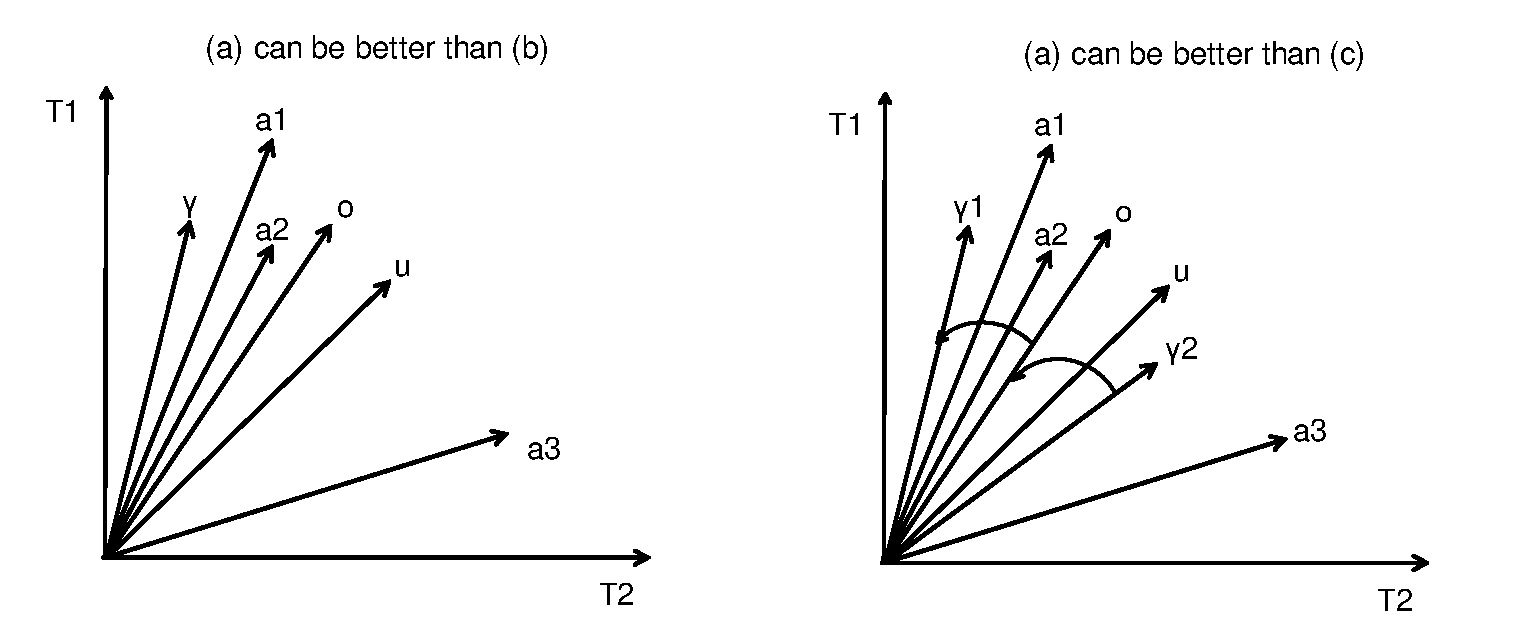
\epsfig{file=figures/betterOurs.eps,height=0.9in}} %, width=3in
\caption{Lezanta}
\label{fig:ourVsRocchio}
\end{figure}

Table \ref{tbl:bit} shows ...

\begin{table}[htbp]
\centering
\caption{Element Index}
\label{tbl:bit}
\begin{tabular}{|l|l|l|}\hline
\textbf{URI or SameAs ID}&\textbf{ID Number}&\textbf{Bit Array}   \\\hline \hline
1 (SameAs ID) &1,2,3 & 111 \\ \hline
2 (SameAs ID)  & 2,3 & 011 \\ \hline
dbp:Texas  & 1,2 & 110\\\hline
dbp:Las\_Vegas  & 2,3 & 011\\\hline
en\_wiki:san\_diego &1,3 &101 \\ \hline
\end{tabular}
\vspace*{-5mm}
\end{table}


%------------------------------------------
\section{Concluding Remarks}
\label{sec:Conclusion}


\bibliographystyle{plain}

\bibliography{bib/report}

\end{document}
